\section{Routing}

This chapter will provide a detailed description of the lightning network routing solution proposed by this work. \\
TH proposed solution for the routing problem involves the creation of a new peer-to-peer network that emerges from the establishment of a new protocol the participating nodes conform to. The beginning of the chapter will provide an overview of the protocol where the reader can get a grasp of how the emergent system works, how the nodes interact to achieve their common routing goal and what kind of components a routing client should have to be able to implement the protocol. This will be followed by a full specification of the protocol. \\
The last part of this chapter will focus on how the different components needed by a client work and how they can be efficiently implemented and maintained.

\subsection{Overview}

The main goal of the protocol, as already described by section \ref{ssec:objectives} is to create a more efficient routing solution for the lightning network, this solution is heavily inspired by the ideas behind distance-vector routing described in section \ref{ssec:distancevectorrouting}. In order to find  payment routes, nodes leverage the information they have available in their routing tables, frequently exchanging this information, so to follow the dynamic nature of the network. Instead of associating a destination to the number of hops it takes to get there from a given node like in most distance-vector routing protocols, the protocol associates given destinations to the maximum volume that a payment can have in order to be successful in paying to the destination node or subnet. It can be thought of as a capacity-vector routing protocol, a distributed, one-path, flow problem. \\
The success of the suggested protocol will depend on how well the routing tables in a given node can approximate the maximum capacity for a payment to a payee node, this will itself depend on how successful nodes are in sharing with the network the available capacities of their own channels. \\
In order to achieve the outlined objectives a node will need to build itself a routing table while following the protocol defined in section \ref{ssec:protocol_specification}, a node will also need a way to register itself in the network, while being able to independently verify that other nodes are also registered in the network, this goal can be achieved by leveraging the capacity of the bitcoin protocol while keeping a local node address database. \\
It's interesting to understand that, much like in the internet, bitcoin is following a layered design principle, the bitcoin protocol stack can be thought as currently composed by the bitcoin protocol serving as a base layer with the lightning network on top of it. As described by figure \ref{fig:bitcoin_protocol_stack} the new suggested protocol, which will be referred from now on as lighting capacity routing protocol or "LCRP" would work on top of lighting as a third layer of the bitcoin stack.

\begin{figure}[H]
\begin{center}
  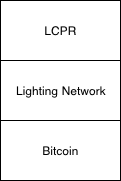
\includegraphics[width=0.2\linewidth]{images/bitcoin_protocol_stack.png}
  \caption{Bitcoin protocol stack (including LCRP)}
  \label{fig:bitcoin_protocol_stack}
  \end{center}
\end{figure}

\subsection{LCRP Specification}
\label{ssec:protocol_specification}

It is important to note that every byte field defined by this specification is Big-endian.

\subsubsection{Blockchain synchronization}
\label{sssec:blockchain_sync}

In order to synchronize itself with the rest of the network a node starts by scanning the bitcoin blockchain from the last analyzed block until the end of the chain. A node should scan the blockchain for transactions whose outputs include a LCRP address registration. An example of one of this outputs is as follows:

\begin{verbatim}
{
        "value" : 0.00000001,
        "n" : 0,
        "scriptPubKey" : {
            "asm" : "OP_RETURN 6c617200000000205fbfaa862899ea7969b9c728fa066834849ef29760036ba0378fc557d6bc17847f24784fc767cc1abd439567bb2d95fb4f4cbc7bc9bbee7430020725a2c5e523",
            "hex" : "6a486c617200000000205fbfaa862899ea7969b9c728fa066834849ef29760036ba0378fc557d6bc17847f24784fc767cc1abd439567bb2d95fb4f4cbc7bc9bbee7430020725a2c5e523",
            "type" : "nulldata"
        }
}
\end{verbatim} 

Taking a close look at the hexadecimal version of the scryptPubKey present in this output helps us understand what is happening here. The first byte represent by 0x6a represents the OP\_RETURN opcode. This byte if followed by 0x48, a byte which represents the length of the rest of the bytes in the scriptPubKey. The  next three bytes exist in order for clients to be able to distinguish this OP\_RETURN output from another unrelated outputs that might also use the OP\_RETURN opcode in their locking script. The hexadecimal representation for this three bytes is "6c 61 72", ASCII for "lar" or "lighting address registration", this helps clients distinguish address registrations from other OP\_RETURN transactions. Then. one byte is reserved for protocol versioning, followed by the next four bytes representing the address that is being registered. In this case, and as an example, we are registering the address 0x00000000 which, using the IPv4 address representation format translates to "0.0.0.0". The last 65 bytes represent a signature, who should have the following properties:

\begin{itemize}
  \item Derived using ECDSA
  \item The ECDSA elliptic curve follows secp256k1 parameters
  \item Is public key recoverable
  \item Signs the SHA-256 hash of the registered address
\end{itemize}

This signature should be represented in accordance to the specification layed out by \cite{libsecp256k1}, the first 64 bytes are divided equally between the (R,S) pair and the last byte is the recovery id.

 The entire scryptPubKey format is represented by table \ref{table:reg_format}. \\

\begin{table}[H]
\label{table:reg_format}
\begin{tabular}{|l|l|l|}
\hline
\rowcolor[HTML]{C0C0C0} 
Field Size (bytes) & Description & Comments \\ \hline
1 & OP\_RETURN opcode & should be set to 0x6a \\ \hline
1 & OP\_PUSHDATA1 opcode & should be set to 0x4c \\ \hline 
1 & length of the information to be pushed into the stack & should be set to 0x4c representing 76 bytes \\ \hline
3 & protocol identifier & identifies the output as an address registration output \\ \hline
4 & protocol version & versioning byte \\ \hline
4 & address & address to be registered \\ \hline
65 & signature & hash of the address signed by the registering node\\ \hline
\end{tabular}
\caption{ScryptPubKey Address Registration Format}
\end{table}

Every new address that was found via scanning the blockchain should then be locally validated and added to the local address database. The address validation rules are the following: \\

Let N be the node registering the address
\begin{enumerate}

\item The format of the address registration scryptPubKey should be of the form: OP\_RETURN opcode + data length + registered address + N's signature.
\item The signature in the address registration output should be a valid signature of the registered address, signed by N, using it's node id.
\item The registered address should be the first unregistered, succeeding address, of an address that belongs to a node that shares a public channel with N or, if N doesn't share at least one public channel with a registered node, be an unregistered address.

\end{enumerate}

Locally validating the registration of every address allows for the existence of a decentralized and eventually consistent address database which does not rely on a central authority for its own existence and maintenance. Although it would be simpler to use a centralized scheme to maintain an address database, this solution maintains the inherit decentralization of the bitcoin protocol stack while also offering a bigger degree of security against all types of attacks that only a centralized solution would be vulnerable against. \\
Thie address validation rules were designed in order to promote the health of the network. By assigning new addresses based on the addresses of the neighbourhood a relation between a nodes address and their position in the network graph is created. This address assigning method takes inspiration from its centralized version, consisting of the assignment of blocks of addresses by a centralized authority to interested parties. This solution promotes the existence of routing tables with a smaller number of entries who can be grouped together by the use of address masking, much like what it is already done today by the routing tables implemented to support the distance-vector routing protocols mentioned in section \ref{ssec:distancevectorrouting}. \\
The OP\_RETURN opcode marks the transaction output as invalid and since any outputs with OP\_RETURN are provably unspendable, some nodes might prune them from the UTXO set, it is of utmost importance that the bitcoin client that is serving the routing service does not prune OP\_RETURN outputs. There is also a limitation, put in place by the relay standards used by most bitcoin clients, setting a limit of 83 bytes for OP\_RETURN scripts, in this case that would mean that the system can fill 81 bytes of data, saving 1 byte for the OP\_RETURN opcode and 1 byte for the data length, this fact should be kept in mind when working with this type of scripting.

\subsubsection{Connecting with Peers}

After scanning the bitcoin blockchain until the last produced block and updating its address database, a node starts constructing its peer list. A node is only able to become peers with nodes who own a registered address and share a lightning network channel with them. All the other nodes, even the other lightning network registered peers whose channels do not include a channel with this node will be invalid LCRP peers. \\
Peer's IP addresses can be found through a request to a lightning network. From there a TCP connection with each one of the peers can be started and maintained. Port 8965 should be used.

\subsubsection{Sign and Authenticate Messages}

Every message sent between LCRP nodes should be signed using the senders private key, appended to the resulting signature and then encrypted using the receivers public key. The first thing a node does after receiving a message is decrypting it using its own private key and verify that it includes a valid signature by one of the neighbouring nodes with a registered address. \\
Signatures should have the following properties:

\begin{itemize}
  \item Derived using ECDSA
  \item The ECDSA elliptic curve follows secp256k1 parameters
  \item Signs the SHA-256 hash of the message
\end{itemize}

Like the signatures of the transaction output scryptPubKey in section \ref{sssec:blockchain_sync}, message signatures conform to the specification layed out by \cite{libsecp256k1}, the first 64 bytes are divided equally between the (R,S) pair and the last byte is the recovery id. \\
The signature is then appended to the signed message and the whole message is encrypted. The encryption process has the following properties:

\begin{itemize}
  \item Uses the ECIES
  \item The ECIES elliptic curve follows secp256k1 parameters
  \item Encrypts the concatenation of the message with its corresponding signature
\end{itemize}

The encrypted message is then appended to its length and can be sent through the network buffer. The byte-format of this message is as follows:

\begin{table}[H]
\begin{tabular}{|l|l|l|}
\hline
\rowcolor[HTML]{C0C0C0} 
Field Size (bytes) & Description & Comments                            \\ \hline
2 & length & length of the encrypted data (uint16) \\ \hline
variable & encrypted data & output of encrypt( message $\|$ sign(message) ) \\ \hline
\end{tabular}
\end{table}

\subsubsection{Message Format}

In order to communicate with it's peers, a node should follow a standard message format, this format is defined as follows:

\begin{table}[H]
\begin{tabular}{|l|l|l|}
\hline
\rowcolor[HTML]{C0C0C0} 
Field Size (bytes) & Description & Comments                            \\ \hline
2                  & type        & 2 bytes indicating the type of message (uint16) \\ \hline
variable           & payload     & a payload that conforms to type           \\ \hline
\end{tabular}
\end{table}

\subsubsection{Building the Routing Table}
\label{sssec:build_table}

When the first successful connection with a peer is established nodes can start building their own locally maintained routing table. To do this a node sets the message type to 0, sending it with an empty payload. The receiving node should answer with a message that includes its own routing table and set the message type byte to 1. So the payload must be of the form:

\begin{table}[H]
\begin{tabular}{|l|l|l|}
\hline
\rowcolor[HTML]{C0C0C0} 
Field Size (bytes) & Description & Comments                                                                               \\ \hline
2                  & count       & 2 bytes indicating the number of entries in the routing table             \\ \hline
4*count            & entries     & byte stream of 4 byte addresses                                          \\ \hline
8*count            & max\_values & byte stream of 8 byte max capacity values for the corresponding addresses \\ \hline
\end{tabular}
\end{table}

This routing table is then analyzed and the relevant information is added to the senders table. The way in which on routing tables are updated with new relevant information is dissected by section \ref{sssec:updateroutingtable}.

\subsubsection{Routing Gossip}

It is through routing gossip messages that the node's local routing table will be maintained with updated routing information. Besides updating the routing tables this messages also work as a "still alive?" system, informing nodes on its neighbors reachability. It is of most importance that gossip messages are periodically sent, with a 60 second period. This messages are characterized by happening after the initial routing table sharing and by having the message type set to 2, including a payload referencing the bitcoin block height the peer's table is synchronized with. The payload has the form:

\begin{table}[H]
\begin{tabular}{|l|l|l|}
\hline
\rowcolor[HTML]{C0C0C0} 
Field Size (bytes) & Description & Comments                                                                               \\ \hline
2                  & count       & 2 bytes indicating the number of entries in the routing table            \\ \hline
4*count            & entries     & byte stream of 4 byte addresses                                         \\ \hline
8*count            & max\_values & byte stream of 8 byte max capacity values for the corresponding addresses \\ \hline
\end{tabular}
\end{table}

\subsubsection{Routing Requests}

The whole point of the LCRP is to be able to route payments from a payer to a payee and routing requests are the backbone of this feature. Every time a node wants to find a payment route to another node it starts by sending a routing request to the selected next hop, this is done by setting the message type to 3, finding the next hop by following the selection rules laid out by section \ref{sssec:selectnexthop} and sending a message conforming to the following payload scheme: \\

\begin{table}[H]
\begin{tabular}{|l|l|l|}
\hline
\rowcolor[HTML]{C0C0C0} 
Field Size (bytes)   & Description          & Comments \\ \hline
4 & destination\_address & 4 bytes indicating the destination address \\ \hline
32 & pubkey & 256 bit public key \\ \hline
105 & source\_address & ( source\_address $\|$ 4 byte salt ) encrypted using receivers public key \\ \hline
2 & path\_len & 2 bytes indicating the length of the path (in bytes) \\ \hline
path\_len & path & output of encrypt( next hop $\|$ max\_value $\|$ previous\_path ) \\ \hline
\end{tabular}
\end{table}

The fields corresponding to the destination address, public key and source address are to be set by the node requesting the route and maintained while the request is being routed. The ECDSA 256 bit private key used to compute the public key field should be stored and used to later decrypt the path. The source address should be set to the 105 byte ECIES encryption of the concatenation of 4 byte sender's address with a 4 byte salt, encrypted using the receiver's node public key.
Each routing request will have different path field, this field should be set to the encrypted representation of the message "next hop $\|$ max\_value $\|$ previous\_path" or, if the node sending the message is the one requesting the path, should be the representation of the message "next hop $\|$ max\_value". The encryption process should respect the following properties:

\begin{itemize}
  \item Uses the ECIES
  \item The ECIES elliptic curve follows secp256k1 parameters
  \item Encrypts "next hop $\|$ max\_value $\|$ previous\_path" or, if node is the first in the path "next hop $\|$ max\_value"
  \item Uses the public key from the field "pubkey"
\end{itemize}

Routing requests are sent from node to node until the address of the receiving node matches the destination address.
When a node processes a routing request that has his own address as the destination\_address it should decrypt the source\_address field and obtain the address of the sender node. The node should then connect to the sender's node and send a type 4 message, the payload will include the path field present in the received routing request:

\begin{table}[H]
\begin{tabular}{|l|l|l|}
\hline
\rowcolor[HTML]{C0C0C0} 
Field Size (bytes) & Description & Comments                                                                       \\ \hline
2                  & path\_len   & 2 bytes indicating the length of the path (in bytes)                           \\ \hline
path\_len          & path        & encrypted path \\ \hline
\end{tabular}
\end{table}

Upon receiving this message the node that originally asked for a path by sending the first routing request decriptes the path field value encrypted layers, extracting the path, hop by hop. When the decryption process ends the node will be left with a path of addresses to the destination and a maximum capacity for the path, given by the minimum max\_value found in the path. This path can then be used to build lightning payments, with an a priori knowledge of the maximum payment amount supported by the route.

\subsection{Address Database}
\label{ssection:add_db}

This section will describe how the address database can be implemented in an efficient way. \\
The address database can be implemented as a binary prefix tree, with a height of 33 if leaves are storing 4 byte addresses. Every time a new address is added a new leaf and its path should also be added to the tree. This data structure optimizes the operations needed to support validation of the address validation rules, with operational time complexity in the order of $\log{}|V|$, with $V$ being the number of nodes. \\
An example of a binary prefix tree structure representing a simple address database is shown in figure \ref{fig:addr_db_example}.

\begin{figure}[H]
\begin{center}
  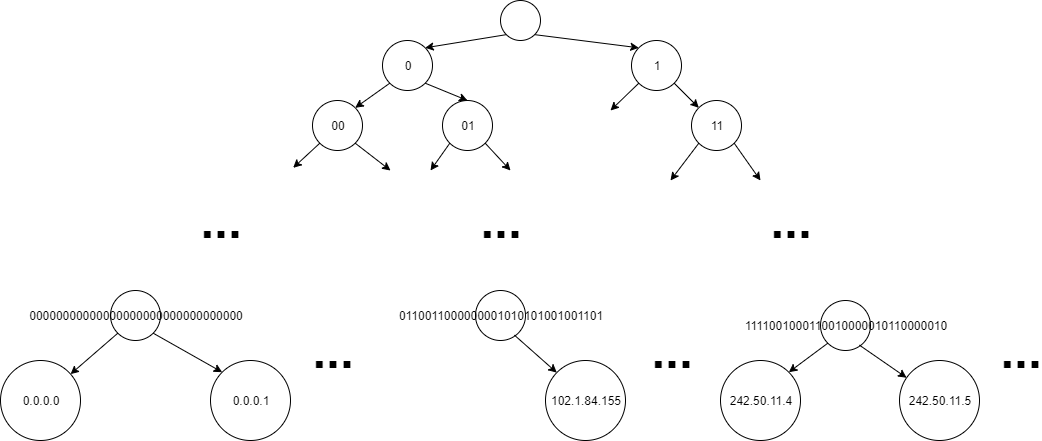
\includegraphics[width=\linewidth]{images/addr_db_example.png}
  \caption{Address Database Example}
  \label{fig:addr_db_example}
  \end{center}
\end{figure}

Nodes higher in the tree represent the most significant bits of the addresses. The database in the figure includes the 4 leaves corresponding to 4 registered addresses and, given that node "01" exists, also includes nodes that are not represented in the figure and whose most significant bits start with "01". Each node that is not a leave always has to have at least 1 child. \\
Let's say that we wanted to follow the address validation rules and register an address for a node that has, as a neighbor, the node with address 0.0.0.1. In order to do this we would go down the tree through the corresponding path from the root to the leaf representing the address 0.0.0.1, from there we could just transverse the tree backwards, using the right children of the transversed nodes as heads for sub trees in which left-to-right DFS's should be done, stopping when the right child doesn't exist or when the DFS finds an non-existing node. The non-existing node and all of its left descendants are then created, creating a leaf with essentially right padding the new address with 0's. From the the validation rules follows that we should always create the left children first, only choosing the right child when the left one is already taken. \\
Figure \ref{fig:reg_addr_db_example} is an example of how a node that has 0.0.0.1 as a neighbour registers the address "0.0.0.3" while confirming to validation rules. The algorithm transverses the nodes in the path from the neighbour address to the root of the tree as depicted by the blue arrows, for every node it tests if it has a right child, if it doesn't the new address will be the node's right child's name right padded with 0's to a 32 bit limit, corresponding to the address of the newly created leaf. If the node has a right child it becomes the head of the sub-tree in which a left-to-right DFS is applied. When the DFS finds the first non-existing child it creates the child and all of its left descendancy, essentially creating a leaf representing the address represented by the child's name right padded with 0's to a 32 bit limit. This process is depicted by the red arrows, in the special case in which the non-existing child is already a leaf.

\begin{figure}[H]
\begin{center}
  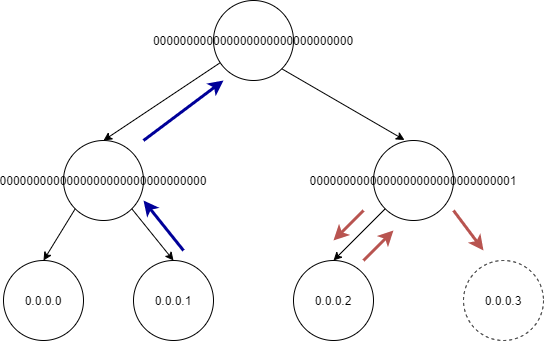
\includegraphics[width=0.8\linewidth]{images/reg_addr_db_example.png}
  \caption{Address Registration Example}
  \label{fig:reg_addr_db_example}
  \end{center}
\end{figure}

The registration can be independently verified by all the nodes on the network using the validation rules and their local binary tree database. Nodes that don't follow the validation rules for registration are not added to the database and consequentially cannot take part in the routing process. \\

\subsection{Routing Tables}

Routing tables serve the purpose of storing information that relates destinations to their next hops and maximum path capacities. They are to be consulted every time a routing request or routing gossip message is sent, so it is important for reading operations to be done efficiently. An efficient way of representing a routing table is with the help of a binary prefix tree similar to the one suggested for the address database data structuring in section \ref{ssection:add_db}. A joint database structure could also be used. \\
The big difference between the trie used to represent the routing table and the one used to represent the address database is that in the former the information to look for might be present in an internal node of the trie while in the latter the information is in the leaves (nodes representing the addresses), with the rest being dummy nodes. The reason for the fact that some internal nodes also store information has to do with the way the addresses and their respective netmasks are stored. Figure \ref{fig:reg_addr_db_example} shows an example of a routing database implemented using a binary prefix tree.

\begin{figure}[H]
\begin{center}
  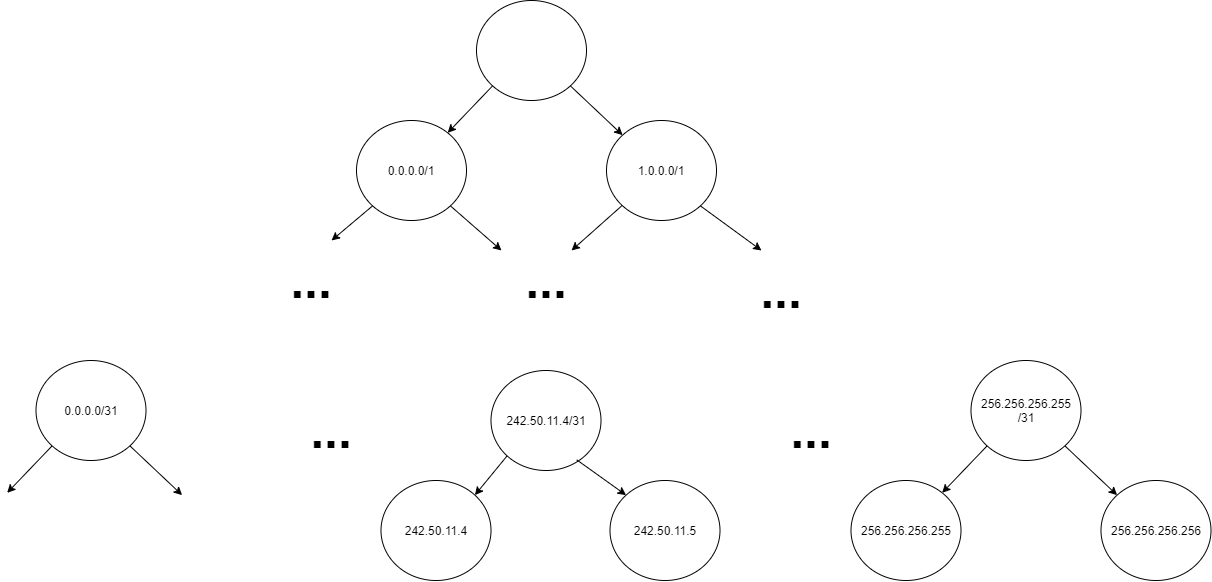
\includegraphics[width=0.8\linewidth]{images/routing_db_example.png}
  \caption{Routing Table Example}
  \label{fig:reg_addr_db_example}
  \end{center}
\end{figure}

Node 0.0.0.0/31 has no children so it must contain some routing information on that specific subnet, node 0.0.0.0/1 might be just a dummy node to support the path to node 0.0.0.0/31 or it might contain information on on subnet with the same name. Contrarily to what happens in the tree that stores addresses, nodes that are not leaves don't need to have any children. \\
The protocol does not specify how or even if the new information should be added to the routing table. This allows for independent implementations of routing table schemes and next hop decision algorithms, words can choose to have smaller routing tables or make their next hop decisions not solely based on the capacity of the path.

\subsubsection{Updating the routing table}
\label{sssec:updateroutingtable}

When receiving routing gossip messages, nodes need to update their routing tables with the new information they receive. New information on destinations and their respective capacities is integrated with the locally kept routing table, the information to be integrated is of the form:

\begin{table}[H]
\begin{tabular}{|l|l|}
\hline
\rowcolor[HTML]{C0C0C0} 
Destination     & Capacity \\ \hline
195.56.13.1     & 6449800  \\ \hline
32.136.89.88/29 & 12933    \\ \hline
\end{tabular}
\end{table}

With U being the updated capacity of a destination or subnet and O the outbound capacity of the channel associated with the node who sent the gossip message. \\
Now let C = max(U, O). \\
A new (destination, capacity) pair should can added to the routing table according to the following rule: \\
If C is larger than the stored capacity for that destination then the new capacity for that destination is now C and the new next hop is the node who sent the gossip message.

\subsubsection{Selecting the next hop}
\label{sssec:selectnexthop}

When a next hop for a certain destination needs to be selected, whether because a routing request was received or because the node wants to request a route to a node, the routing table is consulted. \\
To select the next hop a node should start at the root of the trie and follow the path corresponding to the destination address until it reaches a leaf or the next node doesn't exist. Each next hop associated to each of the transversed nodes is now a possible selection for next hop. Nodes can choose the next hop that corresponds to the smallest subnet, the one linked with the biggest capacity or implement the next hop selection strategy that's more in line with their routing goals.